\newcommand{\nota}[1]{
  $\bullet$ {\color{red}{#1}}
}

\subsection{Referencia de conectores}
A continuación presentamos una referencia a los conectores utilizados en los diagramas que se presentarán en las siguientes secciones. Los conectores \emph{no-standard} utilizados son especificados más abajo.

\begin{multicols}{2}
\begin{figure}[H]
	\centering
	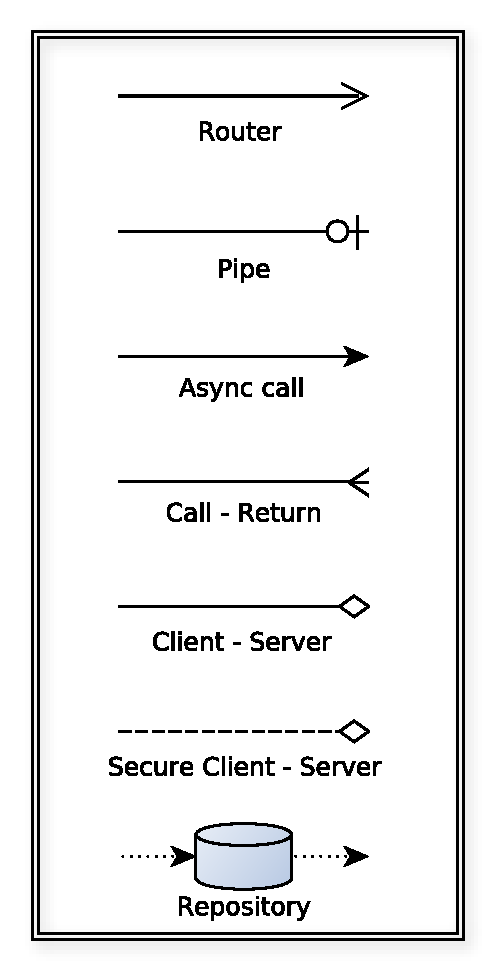
\includegraphics[scale=0.6]{graficos/call_reference.pdf}
	\caption{Referencia de conectores.}
\end{figure}
\begin{figure}[H]
  \centering
  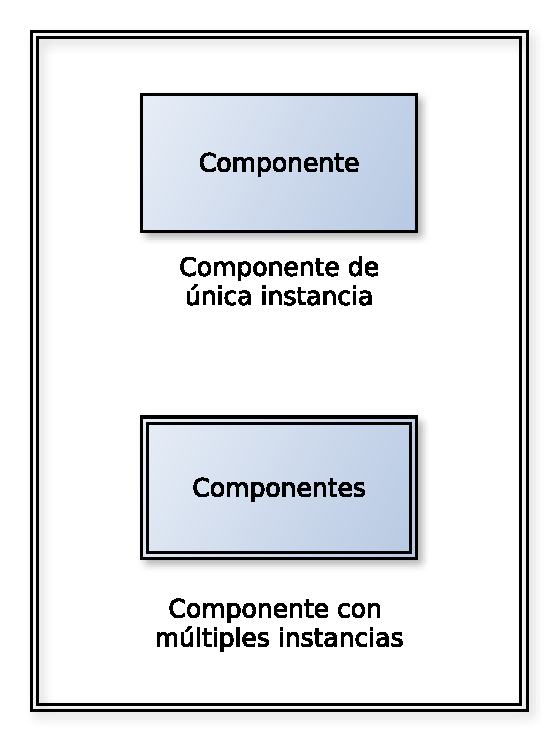
\includegraphics[scale=0.6]{graficos/comp_reference.pdf}
  \caption{Referencia de componentes.}
\end{figure}
\end{multicols}

\paragraph{Conectores no standard}

\begin{itemize}
		%Completar con conectores no standard!
		%Agregar asi:
		\NonStandardConector{A non standard conector name}{A non standard conector description.}
\end{itemize}

\subsection{Conectividad externa del sistema \textbf{TPA}}

En el siguiente diagrama vemos la disposición global del sistema central \textbf{TPA} respecto a los agentes externos con los que interactúa. 

\begin{figure}[H]
	\centering
	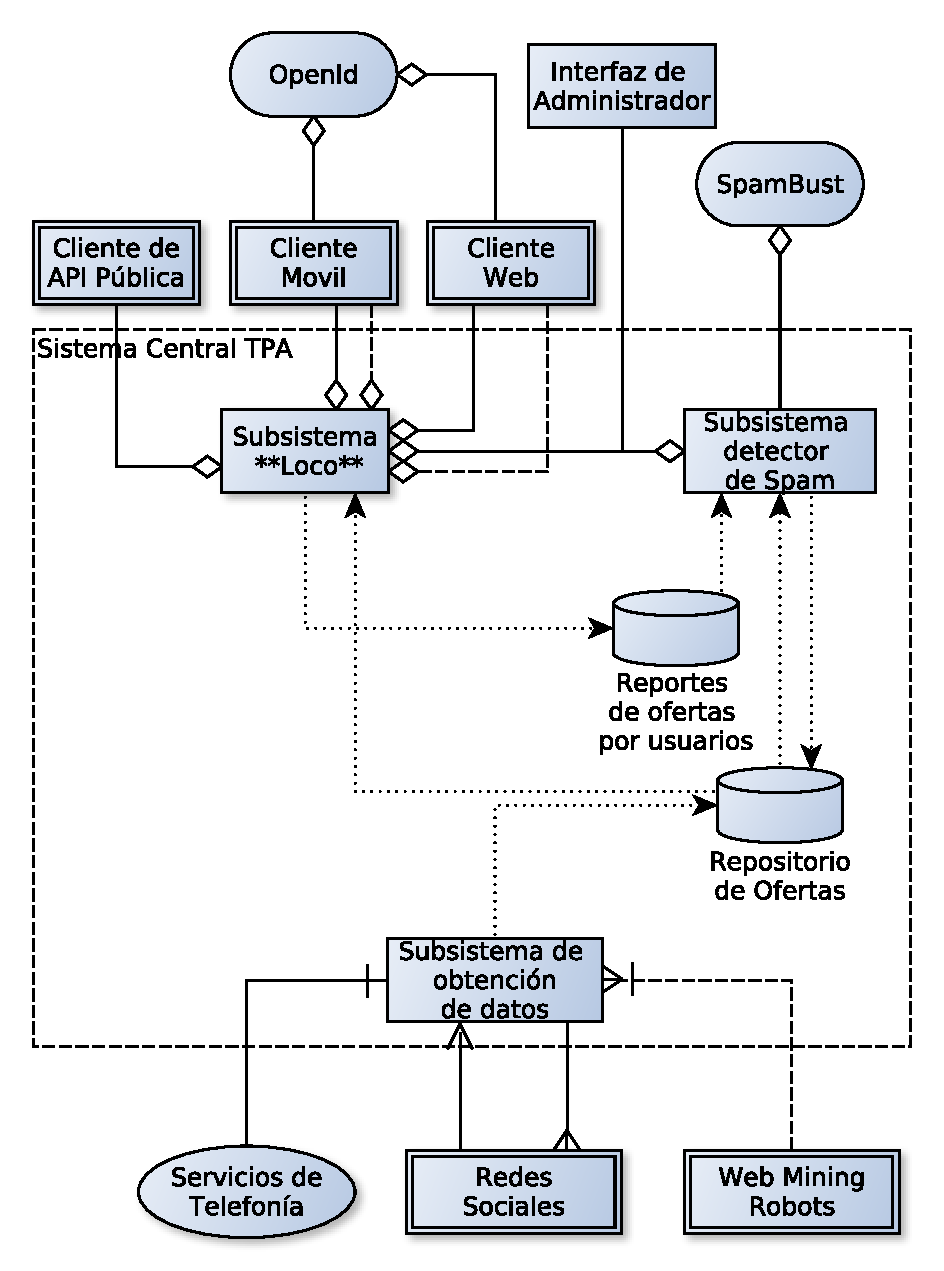
\includegraphics[width=\textwidth]{graficos/arch/global_overview.pdf}
	\caption{Diagrama arquitectónico global del sistema \textbf{TPA}.}
\end{figure}

Aquí vemos al \textsf{Sistema central TPA} dividido en 4 componentes. El \textsf{Subsistema de Ofertas} es el encargado de responder a las consultas de los posibles clientes. En este momento los clientes son nuestras aplicaciones web y móvil, así como aquellos que deseen consumir nuestra API pública. Dentro del \textsf{Subsistema de Ofertas} tenemos los componentes encargados de comprender los pedidos, administrar las preferencias y reputación de usuarios, administrar las publicidades generadas por el sistema, mantener las reglas de asociación y sustitución, y contener la información de los productos y rubros aceptados.

El \textsf{Sist. Obtención de datos} es el encargado de recurrir a las distintas fuentes de datos con el fin de obtener ofertas a productos. Por lo tanto, contiene los medios necesarios para poder extraer información de \textsf{Redes sociales} y para poder recibir información mediante \textsf{SMS}. Como además se decidió poder registrar sitios web con interfaces variadas (muy distintas a las \textsf{Redes sociales}), se cuenta con los componentes \textsf{Web Mining Robots}, que constituyen robots que saben recorrer ciertos sitios específicos en busca de ofertas. El \textsf{Sist. Obtención de datos} sabe cómo comunicarse con los robots, quienes le proveen información. 

Las ofertas obtenidas por el \textsf{Sist. Obtención de datos} le son provistas al \textsf{Subsistema de Ofertas} mediante el uso de un repositorio intermedio.
El mismo es revisado contínuamente por el \textsf{Sist. detector de Spam}, que contiene mecanismos para detectar ofertas de naturaleza dudosa. En este momento, el principal mecanismo es el sistema de terceros \textsf{SpamBust}.

\subsection{Subsistema de Query}

En el siguiente diagrama se presenta el \textsf{Subsistema de Query} donde, dada una consulta por productos (\textbf{query}), se arma la respuesta para el usuario que realizó la consulta. En este diagrama se encuentran ejemplificados los \emph{casos de uso} 7, 8, 9, 10, 11 y 12.

\nota{Revisar CUs}

\begin{figure}[H]
	\centering
	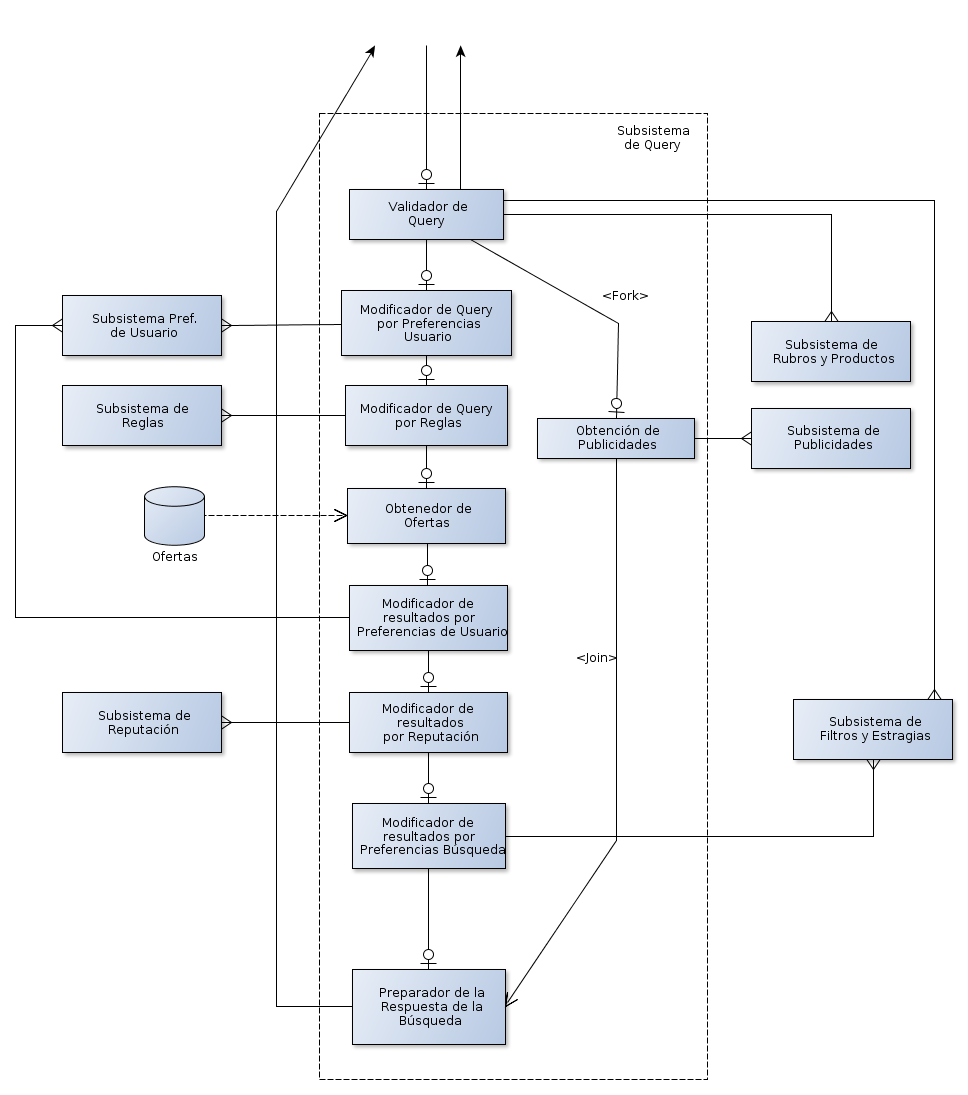
\includegraphics[width=\textwidth]{graficos/arch/subsistema_query.png}
	\caption{Diagrama arquitectónico con el detalle del \textsf{Subsistema de Query}.}
\end{figure}

La funcionalidad de este componente es la de procesar un pedido por productos para armar todo el contenido que le será devuelto al usuario. Este procesamiento incluye varias funcionalidades del sistema. Todas estas pueden realizarse de forma encadenada, lo cual lleva a que el componente trabaje con un estilo arquitectónico de tipo \emph{pipes and filters}, en el cual cada etapa de procesamiento se realiza secuencialmente pero de forma independiente. La elección de este estilo tiene como fin lograr \emph{modificabilidad} y \emph{performance}, ya que las etapas pueden reubicarse sin tener que modificar fuertemente el sistema; además, para aquellas etapas que requieren mayor poder de cómputo pueden agregarse más recursos, de forma que no generen un cuello de botella.

En primer lugar se valida que el pedido sea realizable (i.e.: es de un producto soportado y posee estrategias y filtros del sistema) por el \textsf{Validador de Query}. Dentro de las funcionalidades, se definieron distintas modificaciones que podrían sufrir las consultas. Los siguientes dos componentes (\textsf{Modificador de Query por Preferencias Usuario} y \textsf{Modificador de Query por Reglas}) se encargan de comunicarse con los subsistemas correspondientes que definen como debe realizarse las modificaciones. El validador encola la consulta para que sea procesada por estos componentes y a su vez la encola para que sea trabajada por el \textsf{Generador de publicidades}, que se encarga de generar las publicidades que formarán parte de la respuesta. Esto se realiza con un mecanismo de \emph{fork and join}, donde el \textsf{Generador de publicidades} toma la \emph{query}, la trabaja y luego espera a que sea consultado por el resultado. De esta forma, la generación de propagandas, que se considera 
independiente del resto del procesamiento a realizar, puede realizarse en paralelo, mejorando la \emph{performance del proceso}.

Las modificaciones que se realizan a la consulta están relacionadas con las preferencias del usuario (que puede decidir no ver las consultas provenientes de algunos usuarios) y las reglas de asociación y substitución, (que establecen que distintas extensiones a las búsquedas). La naturaleza de estas modificaciones no está completamente definida pero estará contenida exclusivamente en los \textsf{Subsistema de Preferencias de Usuario} y \textsf{Subsistema de Reglas}. 

Con la consulta (\emph{query}) ya definida y ajustada, el componente \textsf{Obtenedor de Ofertas} accede al repositorio de ofertas y adquiere todas aquellas que responden a la consulta.  Una vez realizado esto pasamos a la etapa donde se prepara el resultado. Por un lado el componente \textsf{Modificador de resultados por Preferencias de Usuario} se encarga de tareas como jerarquizar las ofertas según las preferencias del usuario. Las ofertas luego son decoradas, eliminadas y reorganizadas según la reputación de los usuarios que las originaron (componente \textsf{Modificador de resultados por Reputación}). A continuación se realiza un nuevo trabajo sobre los resultados aplicando los filtros y estrategias seleccionados por el usuario en la consulta original (componente \textsf{Modificador de resultados por filtros y estrategias}). Finalmente, el componente \textsf{Preparador de la Respuesta de la Búsqueda} prepara todo el paquete de respuesta que será enviado denuevo al usuario. 

\subsection{Interfaz móvil}

La interfaz móvil es uno de los componentes encargados de facilitar una interfaz comoda al usuario, y comunicar los pedidos de este con el servidor central de \emph{twitteando para ahorrar}.

A través de este subsistema, el usuario deberia ser capaz de:
\begin{enumerate}
	\item Realizar consultas de ofertas.
	\item Denunciar ofertas como falsas.
	\item Permitir conectarse con una cuenta en un provedor de \emph{OpenId}.
	\item Permitir modificar la configuración del usuario.
\end{enumerate}

Al mismo tiempo, ciertos atributos de calidad guían el diseño de este subsistema. Alguno de ellos son la necesidad de \emph{responder rapidamente al usuario} (¡inclusive antes de que este comience a tipear algo!), y la necesidad de \emph{garantizar disponibilidad}, a pesar de que no exista conexión.

Al modulo de interfaz de usuario se le delega la tarea de presentar los datos de una forma 'bonita y comprensible' al usuario. Además, este modulo se comunica con el componente encargado de facilitar la posibilidad de autenticarse con \emph{OpenId}. Vale destacar que el componente de comunicación con OpenId se encuentra en el cliente y no del lado del servidor, ya que es el \emph{proveedor de OpenId} (\textsf{facebook}, \textsf{linkedin}, etc.) el cual ofrece un formulario para autenticarse. De esta forma, durante la autenticación, el control es cedido al \emph{proveedor de OpenId}.

Por otro lado, la interfaz de usuario se comunica con el modulo que intercambia mensajes con el sistema central de \emph{twitteando para ahorrar}. Se decidió que, tanto los mensajes enviados desde la interfaz al modulo de comunicación, como los del modulo de comunicación a la interfaz de usuario, serán enviados de forma asíncrona. Esta ultima decisión tiene como objetivo evitar 'congelar' la interfaz esperando por una respuesta del servidor. 

\begin{figure}[H]
	\centering
	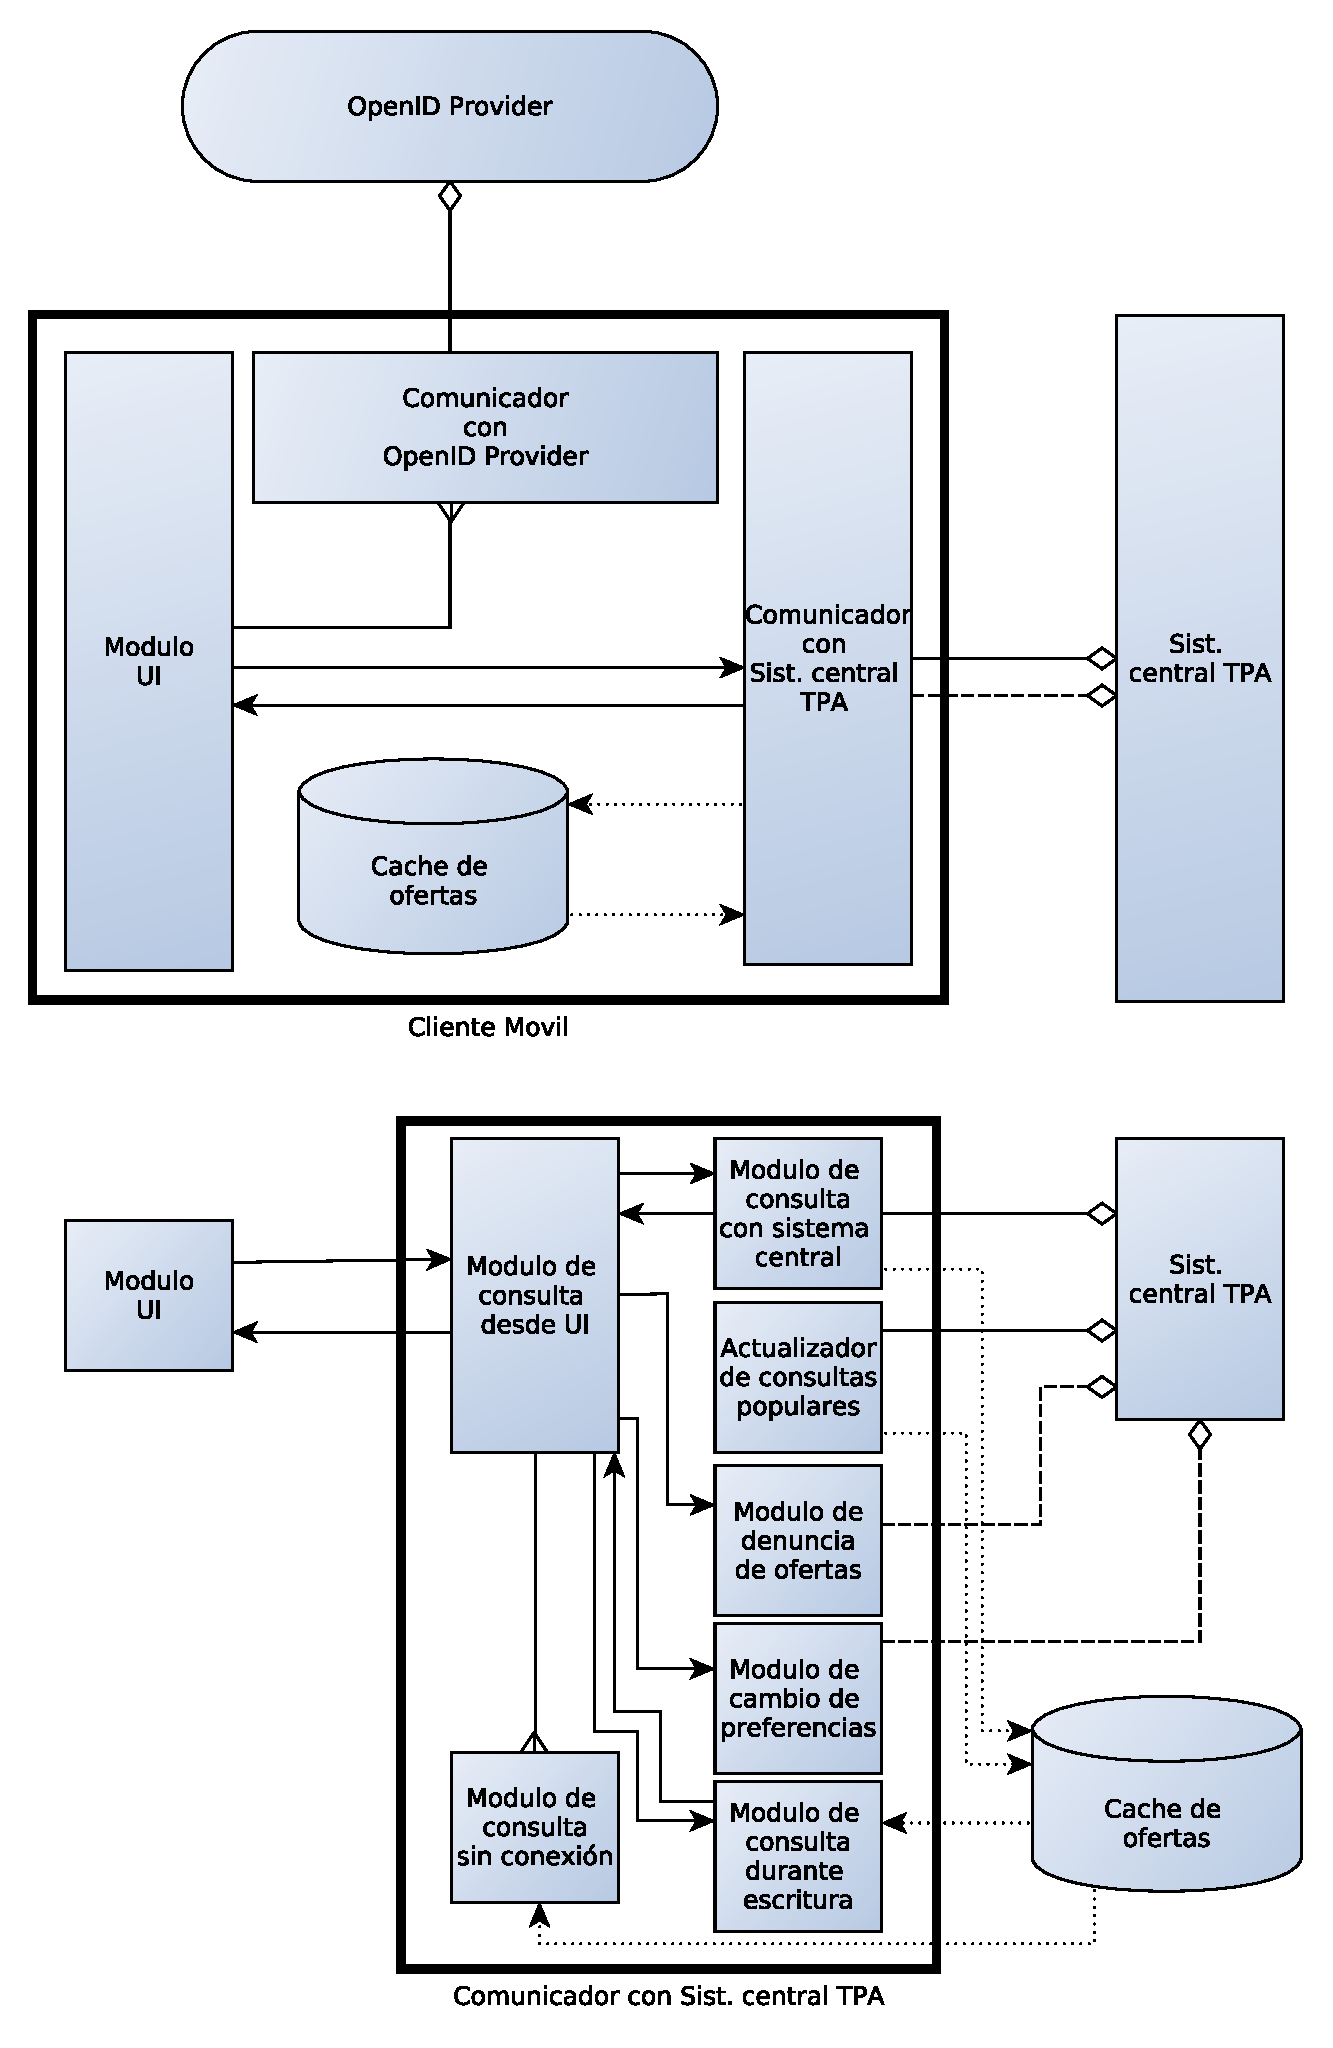
\includegraphics[width=\textwidth]{graficos/arch/Cliente_movil.pdf}
	\caption{Diagrama arquitectónico con el detalle del \textsf{Cliente móvil}.}
\end{figure}

\subsubsection{Modulo de comunicación con el sistema de Twitteando para ahorrar}

Este modulo convierte las ordenes que el usuario envia desde la interfaz grafica, en consultas efectivas por ofertas, entre otras funcionalidades. 

Para comprender el funcionamiento de este subsistema, vamos a plantear el siguiente ejemplo:

\begin{figure}[H]
	\centering
	\emph{Tito Codito, conocido ahorrador, abre la interfaz móvil de Twitteando para ahorrar, desde su smarthphone, y busca por ofertas de \emph{Pepas Tocoñato}\footnote{Muy superiores a las Terepín}.}
\end{figure}

En el momento en el que Tito inicia la aplicación desde su móvil, el \textsf{Modulo de consulta desde UI} realiza una consulta al \textsf{Modulo de consulta sin conexión}, con el objetivo de obtener, de la \textsf{Cache de ofertas}, las ofertas registradas como \emph{Mas populares}. De esta forma, si bién Tito no comenzó a escribir una consulta, resultados interesantes se muestran en la interfaz de usuario. Estas ofertas se mantienen actualizadas en la cache por el \textsf{Actualizador de consultas populares}.

Luego, Tito comienza a escribir la consulta, \emph{Pep}, sin embargo, la interfaz gráfica, registra este evento antes de que la consulta se termine de tipear, y lo informa al \textsf{modulo de consulta desde UI}. Este modulo, consulta al \textsf{Modulo de consulta sin conexión} por consultas sobre productos que empiecen con este patrón. Los resultados son comunicados inmediatamente a la interfaz. Así, resultados son mostrados antes de que la consulta se termine de tipear. La desventaja de esta solución es que solo se pueden 'predecir' resultados de consultas realizadas previamente, o consultas populares. 

Una alternativa que no posee este problema, es realizar esta consulta con el sistema central, sin verificar antes la cache, sin embargo los tiempos necesarios para la transferencia de datos y resultados con el servidor, hacen que esta opción sea inviable, y que una vez que se tienen resultados, Tito ya llevaría un timepo considerable desde haber terminado de escribir la consulta.

Una vez que la interfaz detecta que la escritura de la consulta se ha terminado, se informa al \textsf{Modulo de consulta desde UI}, este resolverá:
\begin{itemize}
	\item Si hay conexión con el servidor central, enviar esta consulta a este servidor y esperar por los resultados. 
	\item En caso de no haber conexión, la consulta se intenta resolver utilizando la cache local.
\end{itemize}

En ambos casos, una vez obtenidos los resultados, estos son enviados a la interfaz grafica para su visualización y, de esta forma, Tito ya puede escoger cuál es el lugar mas conveniente para comprar \emph{pepas}.

De forma ortogonal a esto, existen otros dos subcomponentes de este módulo. Estos son, el \textsf{módulo de cambio de preferencias} y el \textsf{módulo de denuncia de ofertas}. El primero tiene la tarea de, ante un cambio de las preferencias del usuario, comunicarselas al servidor central. El segundo componente, comunica al servidor central la denuncia de una oferta como posible falso. La comunicación de ambos modulos con el servidor se realiza de forma \emph{segura}, debido a que los datos que circulan en este momento son sensibles, y se busca evitar posibles usos malintencionados. Un ejemplo de lo anterior, seria atacar al sistema, denunciando ofertas, haciendose pasar por otro usuario. 

\begin{figure}[H]
	\centering
	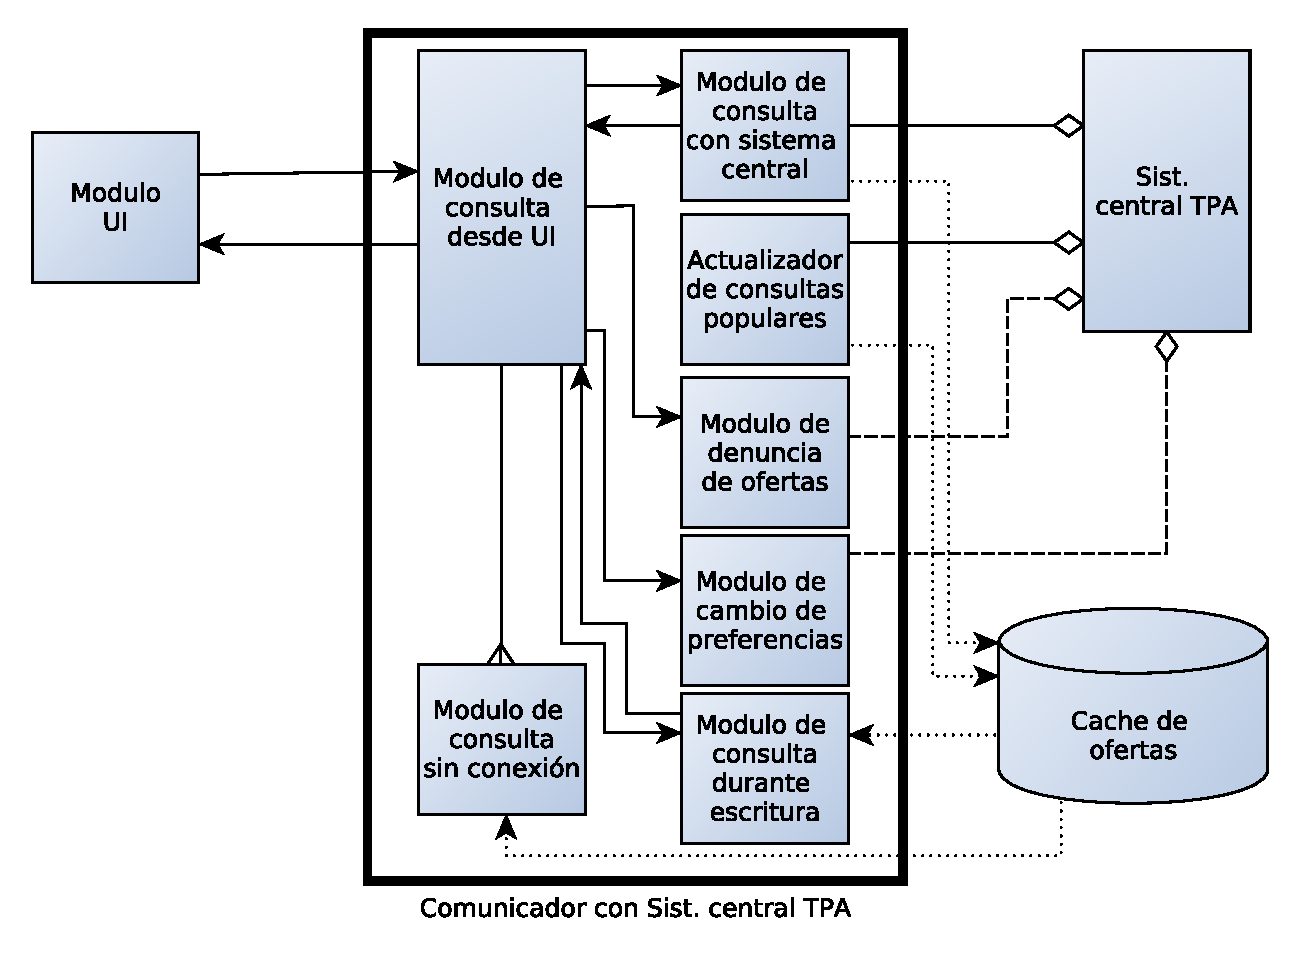
\includegraphics[width=\textwidth]{graficos/arch/cliente_movil_comunicador.pdf}
	\caption{Diagrama arquitectónico con el detalle del \textsf{Comunicador con Sist. central TPA} del \textsf{Cliente móvil}.}
\end{figure}

\subsection{Interfaz web}

De forma similar a la Interfaz móvil, para permitir el acceso desde un conjunto diverso de dispositivos, optamos por dar lugar a una interfaz web de nuestra aplicación.

Esta interfaz se diferencia de la móvil en un punto importante, \textbf{no} se puede \emph{persistir la información} obtenida de consultas anteriores. Esto imposibilita utilizar las estrategias, utilizadas en la interfaz movil, para responder rapidamente a consultas del usuario, mientras estas se escriben. Por el mismo motivo, resulta imposible acceder sin conexión al servicio, sin embargo, es esperable que la misma interfaz sea inaccesible, en ausencia de conexión.

La unica funcionalidad recortada en la interfaz web en comparación con la interfaz móvil es la posibilidad de anticiparse al usuario mientras este escribe la consulta.

Cuando un usuario se conecta a este servicio, al mismo tiempo que se carga la interfaz de usuario, comienzan a obtenerse las ofertas más populares, para sugerirlas por la interfaz, antes de que se comiencen a realizar consultas por otros productos.

Luego, si se realiza una consulta por un producto en particular, esta es delegada al \textsf{Modulo de consultas desde UI}, y de forma sincrónica se realiza la comunicación con el servidor central.

La comunicación entre la interfaz gráfica y el módulo de consultas desde UI se realiza de forma asincrónica, para dar al usuario la sensación de agilidad en la respuesta, y no 'congelar' la interfaz grafica.

\begin{figure}[H]
	\centering
	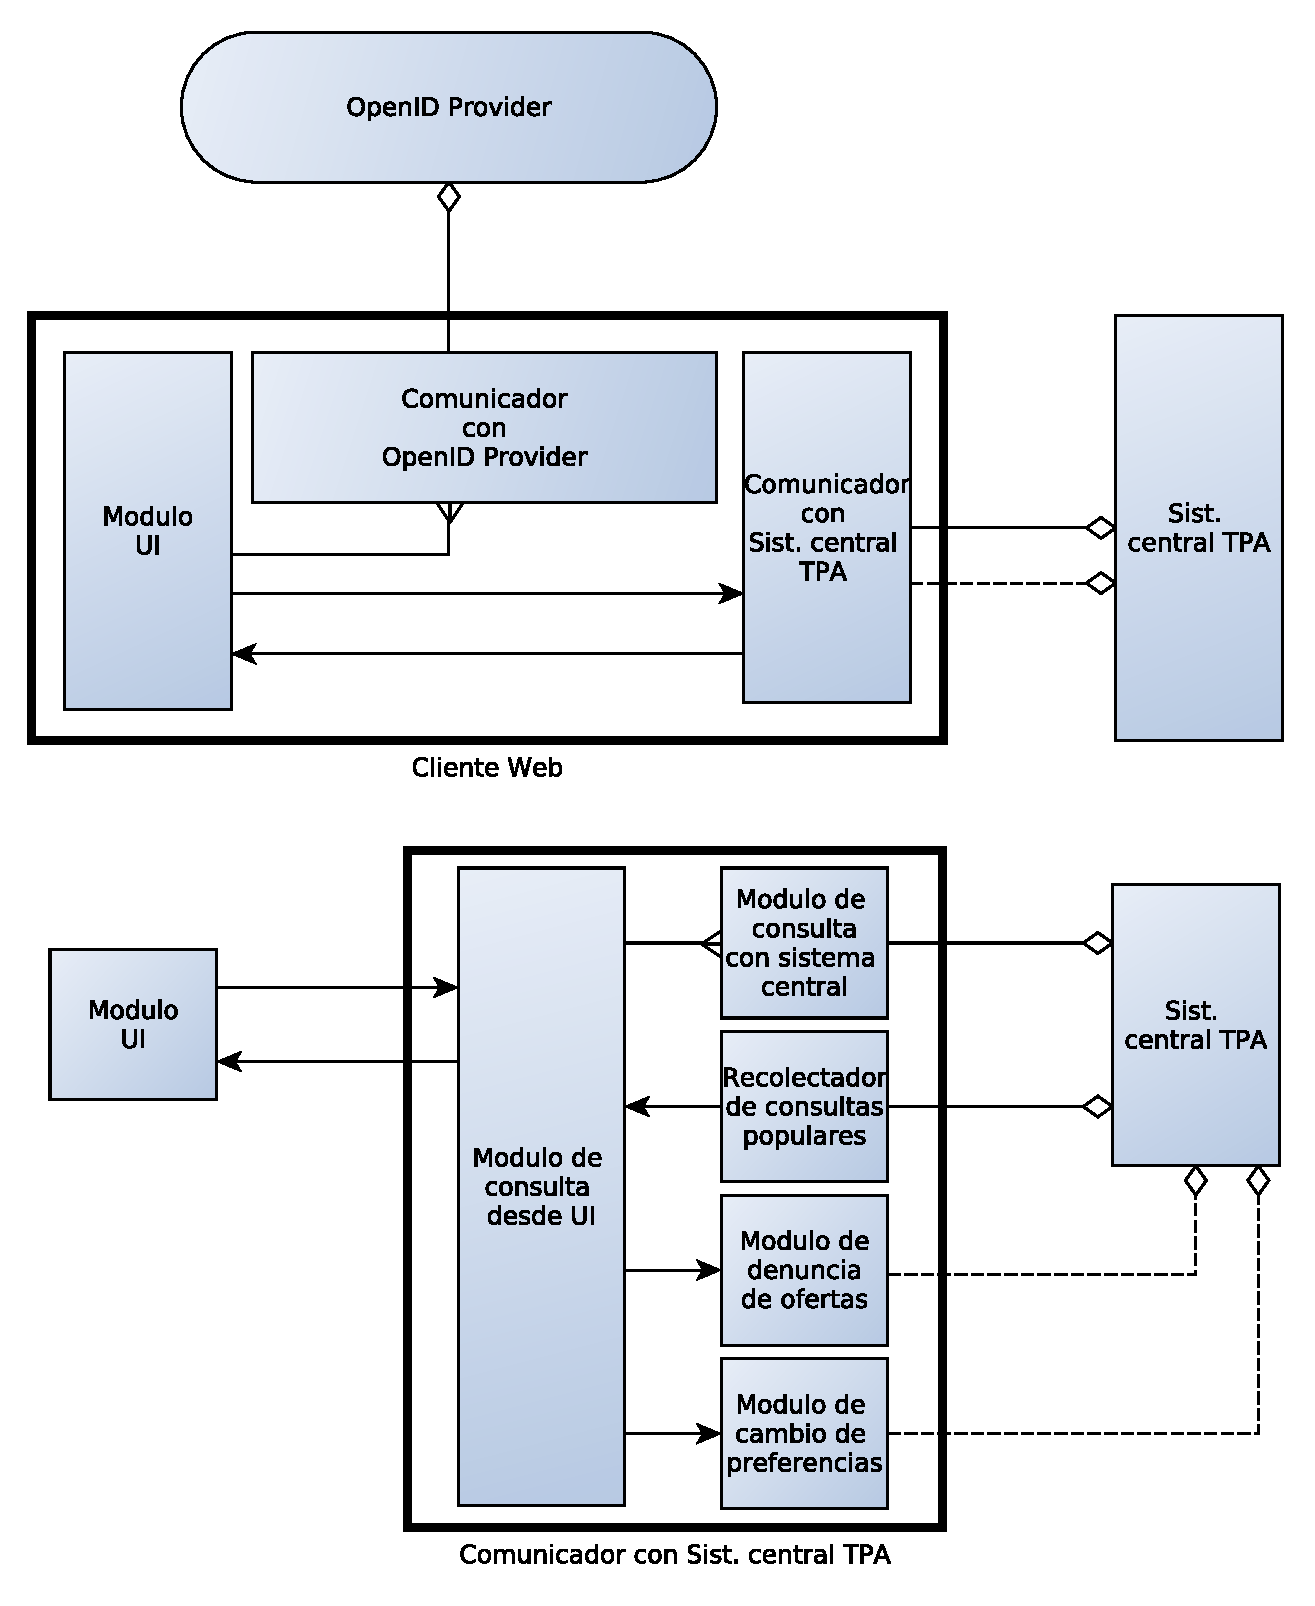
\includegraphics[width=\textwidth]{graficos/arch/Cliente_web.pdf}
	\caption{Diagrama arquitectónico con el detalle del \textsf{Cliente web}.}
\end{figure}


\subsection{Subsistema de Detección de Spam}

El siguiente diagrama representa el Subsistema de Detección de Spam (\textbf{SDS}) donde se discriminan las ofertas deseadas en el sistema de las que no lo son (\textbf{Spam}). El hecho que una oferta sea no deseada puede deberse a que sea falsa, productos con precios dudosos, información contradictoria y/o alerta de enga\~{n}os reportados por los usuarios del sistema.
\nota{revisar la oración anterior}

\begin{figure}[H]
	\centering
	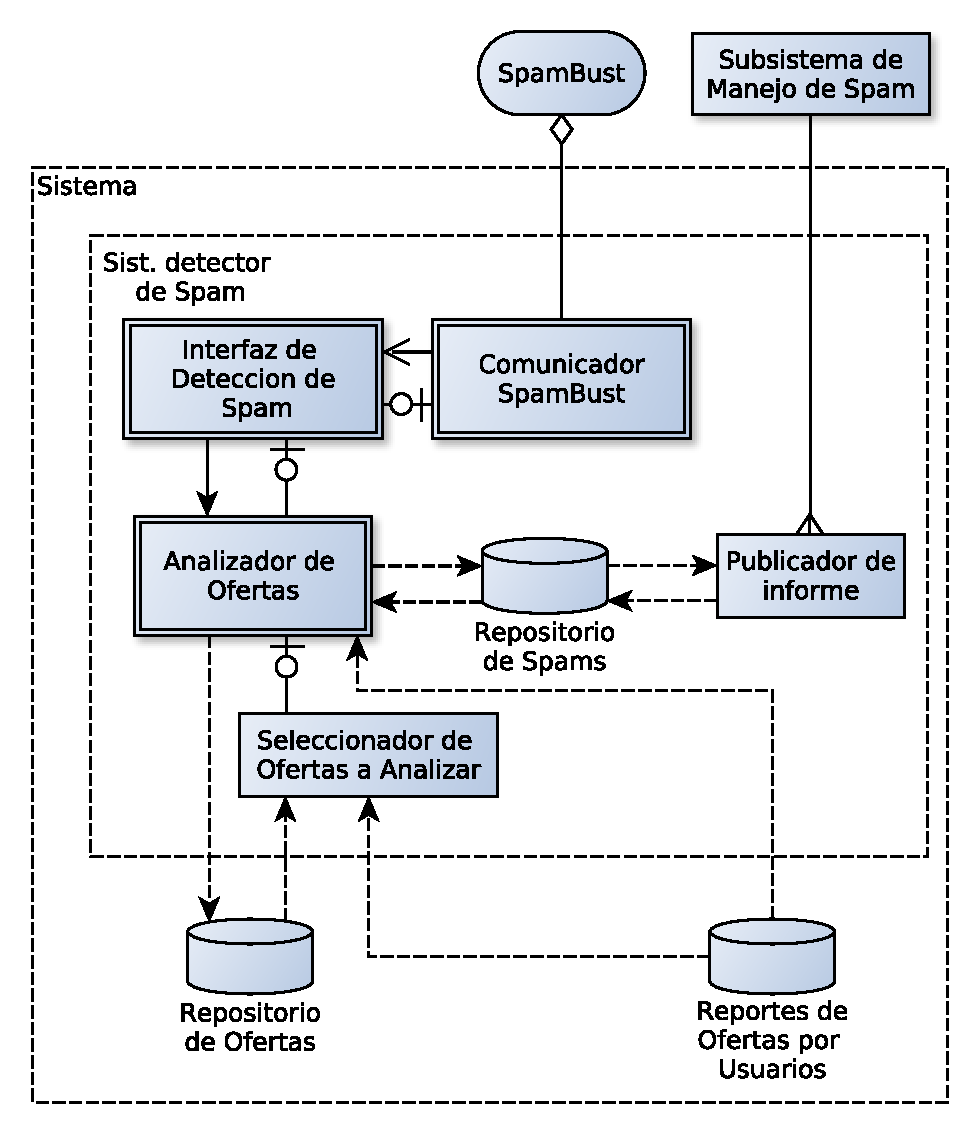
\includegraphics[width=\textwidth]{graficos/arch/Sistema_deteccion_spam.pdf}
	\caption{Diagrama arquitectónico con el detalle del \textsf{Subsistema de Detección de Spam}.}
\end{figure}

El SDS lee constantemente el \textsf{Repositorio de Ofertas} priorizando las ofertas recientemente agregadas que no han sido analizadas nunca como spam y las que fueron reportadas como enga\~{n}osas por los usuarios, de esto se encarga la componente \textsf{Selector de Ofertas a Analizar}. Esta componente le pasa en forma de \emph{pipe} las ofertas seleccionadas a la componente \textsf{Analizador de Ofertas} que se encarga de discernir si la oferta es un spam o no lo es. Por temas de \emph{Performance} se decidió que haya múltiples instancias de esta componente, permitiendo que diversos recursos se ocupen de cada una de estas (\emph{Concurrencia}).\\

El \textsf{Analizador de Ofertas} consideración la respuesta del servicio de \textsf{SpamBust} como también los reportes de usuarios o viejas ofertas detectadas como spam para tomar la decisión final de marcar una oferta como spam. Para la comunicación con los servicios de \textsf{SpamBust} interactúa con un componente \emph{intermediario} llamada \textsf{Interfaz de Detección de Spam} la cual se encarga de transferir los pedidos a la componente \textsf{Comunicador SpamBust} que es el responsable de los detalles específicos de la comunicación con el servicio de \textsf{SpamBust}. Esto concede a la arquitectura una gran \emph{Modificabilidad} ya que el \textsf{Analizador de Ofertas} se comunica solo con un \emph{intermediario} que es fácilmente sustituido/modificado para apuntar a otra componente que no sea el \textsf{Comunicador SpamBust}, como por ejemplo una implementación propia que sustituya los servicios de \textsf{SpamBust}.\\

El \textsf{Analizador de Ofertas} también se encarga de borrar del \textsf{Repositorio de Ofertas} aquellas ofertas encontradas como Spam y guardarlas en el \textsf{Repositorio de Spams} para su posterior revisión/publicación, de esto último se encarga la componente \textsf{Publicador de Informe}.\\

\subsection{Subsistema de Obtención de Datos}


En el siguiente diagrama representa el Subsistema de Obtención de Datos (\textsf{SOD}) el cual se encarga de la interacción con los diversos proveedores de ofertas para alimentar el sistema con estas.\\

\begin{figure}[H]
	\centering
	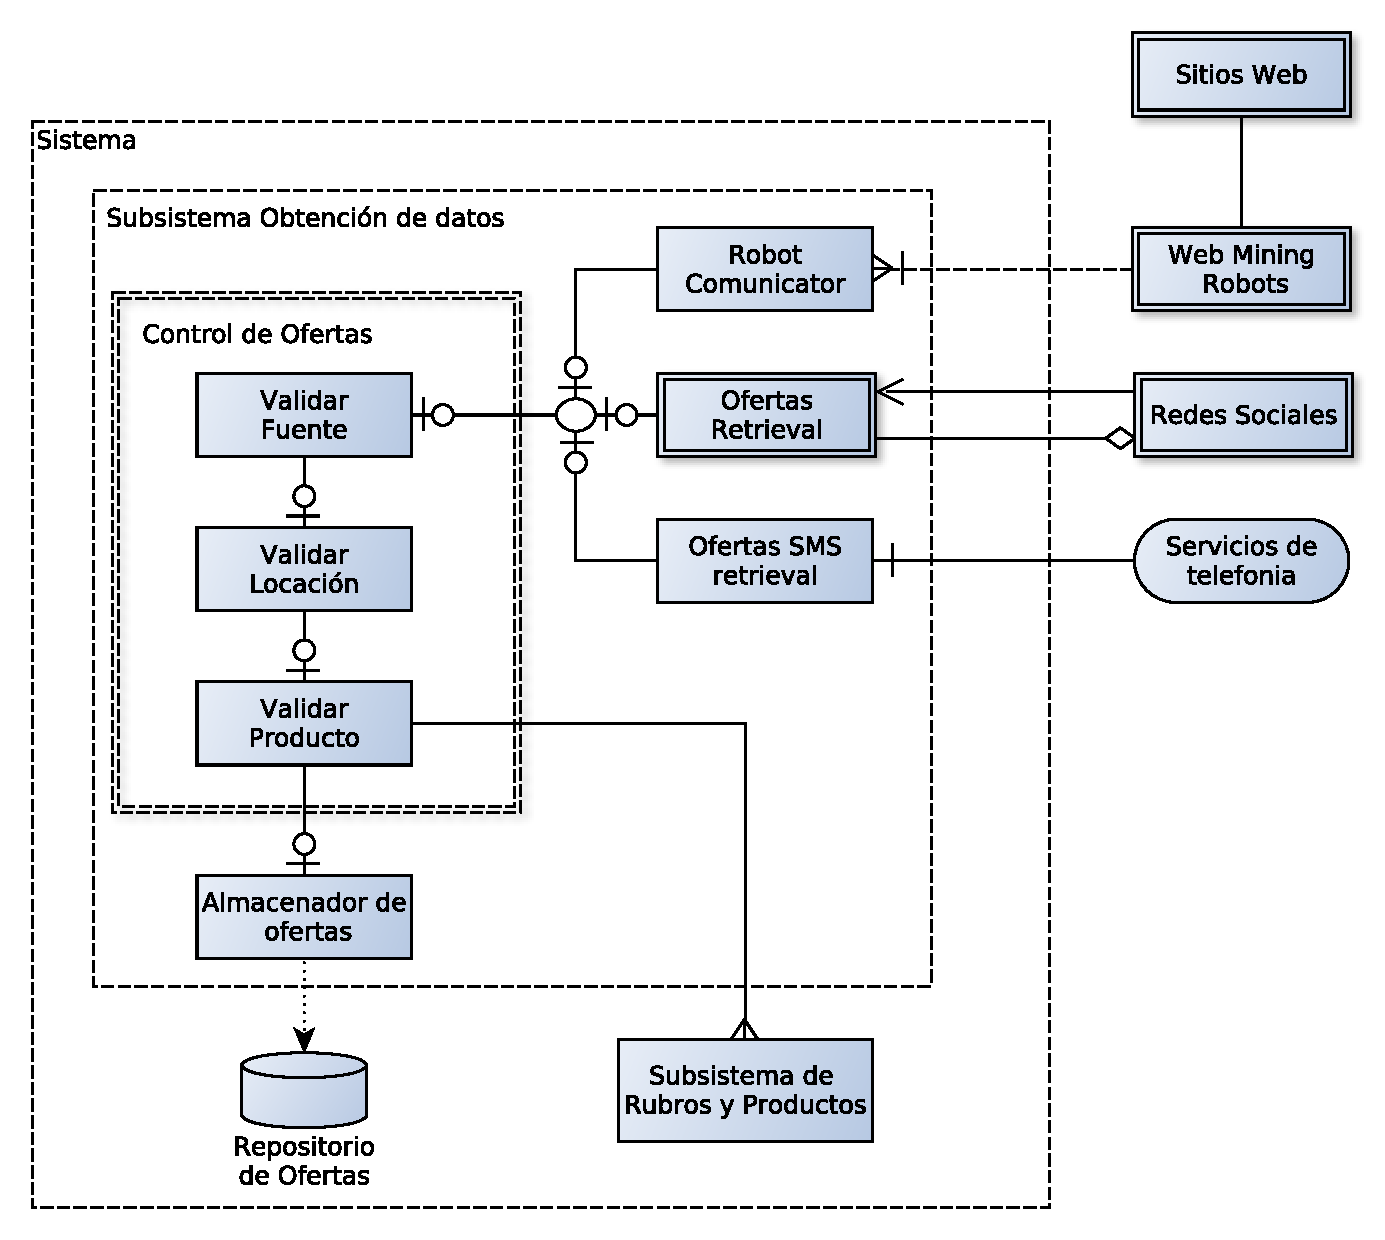
\includegraphics[width=\textwidth]{graficos/arch/Sistema_obtenedor_datos.pdf}
	\caption{Diagrama arquitectónico con el detalle del \textsf{Subsistema de Obtención de Datos}.}
\end{figure}

el SOD se encarga de recolectar datos vía SMS, redes sociales y Web Mining. Cada una de las cuales tiene un componente responsable de interactuar con sus respectivas fuentes de información y colocar las posibles ofertas en una manera genérica para que puedan ser validadas por la componente \textsf{Control de Ofertas}. Esta última componente recibe en forma de \emph{Pipe} la información de las tres componentes encargadas de la interacción con el exterior(\textsf{Robot Comunicator}, \textsf{Ofertas Retrieval} y \textsf{Ofertas SMS retrieval}).\\

La componente \textsf{Control de Ofertas} se encarga de verificar si la oferta es aceptada como validad por el sistema, como esto puede llegar a ser mucho más costoso computacionalmente que la recolección de datos, se tiene múltiples instancias de esta componente para poder soportar \emph{concurrencia}. Para los chequeos usa el estilo \emph{pipe and filter} para que sea fácilmente \emph{Modificable} en el futuro. Una vez que se hacen todos las validaciones pertinentes esta componente le pasa la oferta al \textsf{Almacenador de Ofertas} para que la guarde en el \textsf{Repositorio de Ofertas}.\\


\nota{Nota: la mezcla entre nombre de ingle y espa~nol es cualquiera...}\\
\nota{nota2: que eso eso de cliente servidor asincronico??}\\
\nota{nota3: los robot hay que expandirlos, como?}\\


\subsection{MARCHHHH}

\begin{figure}[H]
	\centering
	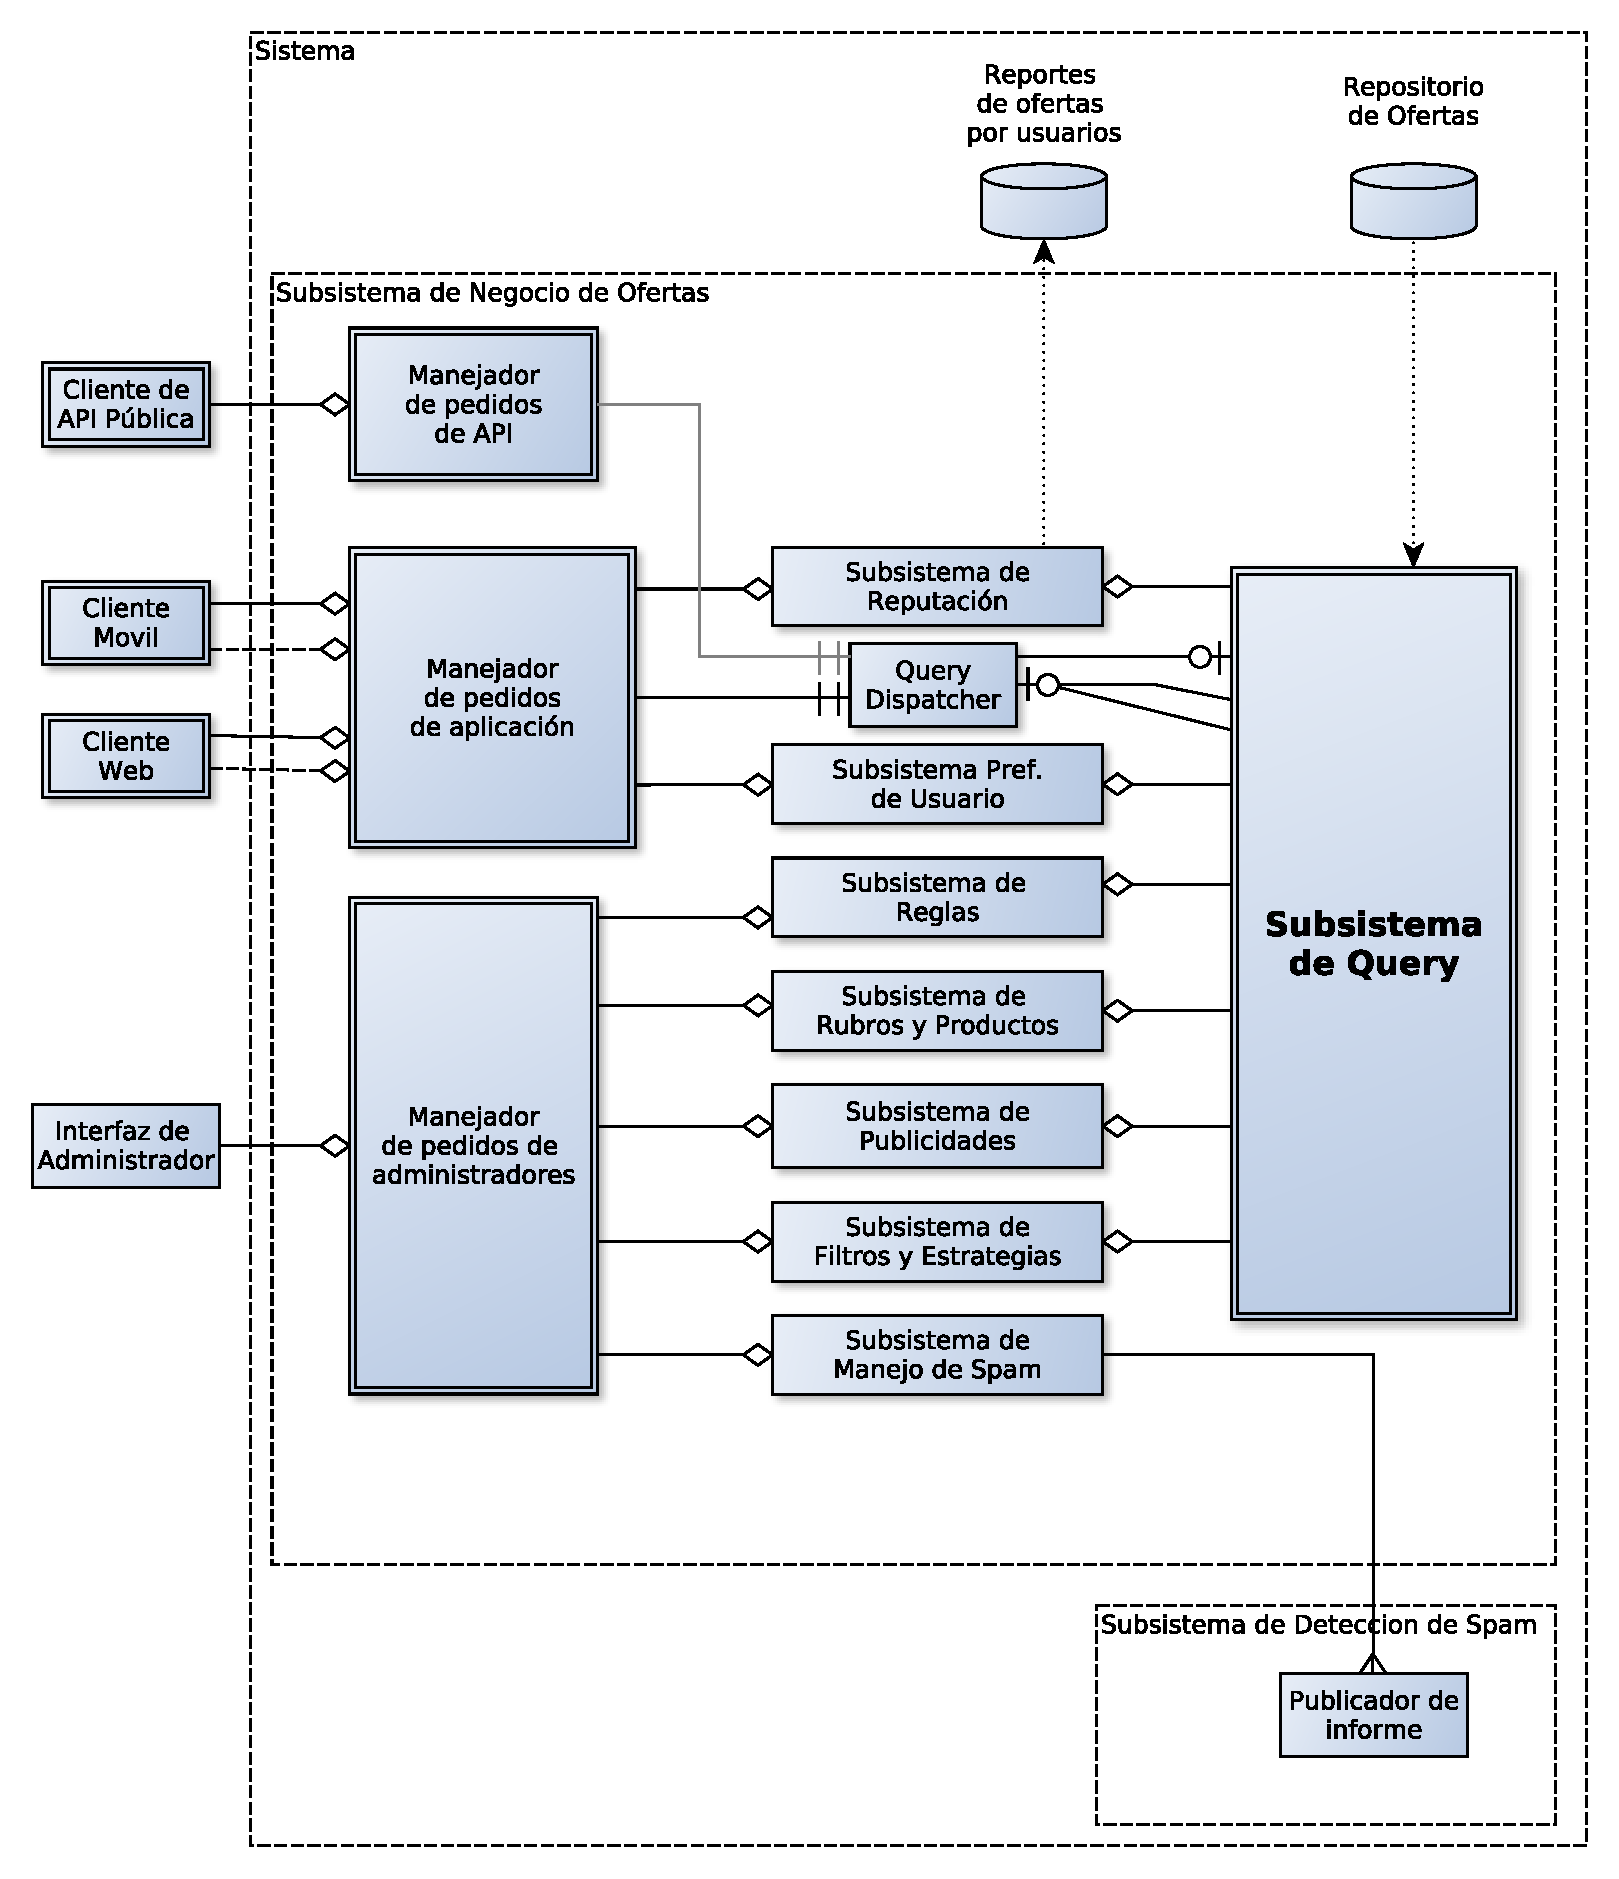
\includegraphics[width=\textwidth]{graficos/arch/temp_subsistema_que_habla_con_el_usuario.pdf}
	\caption{Diagrama arquitectónico con el detalle del \textsf{Subsistema de Obtención de Datos}.}
\end{figure}

